\documentclass[border=10pt]{standalone}
\usepackage{tikz,amsmath,dsfont}
\usetikzlibrary{shapes.geometric, arrows}

\tikzstyle{agent} = [rectangle, 
rounded corners, 
minimum width=2cm, 
minimum height=1cm,
text centered, 
draw=black, 
fill=black!30]
\tikzstyle{arrow} = [thick,->,>=stealth]

\tikzstyle{env} = [rectangle, 
rounded corners, 
minimum width=3cm, 
minimum height=1cm,
text centered, 
draw=black, 
fill=brown!30]

\begin{document}
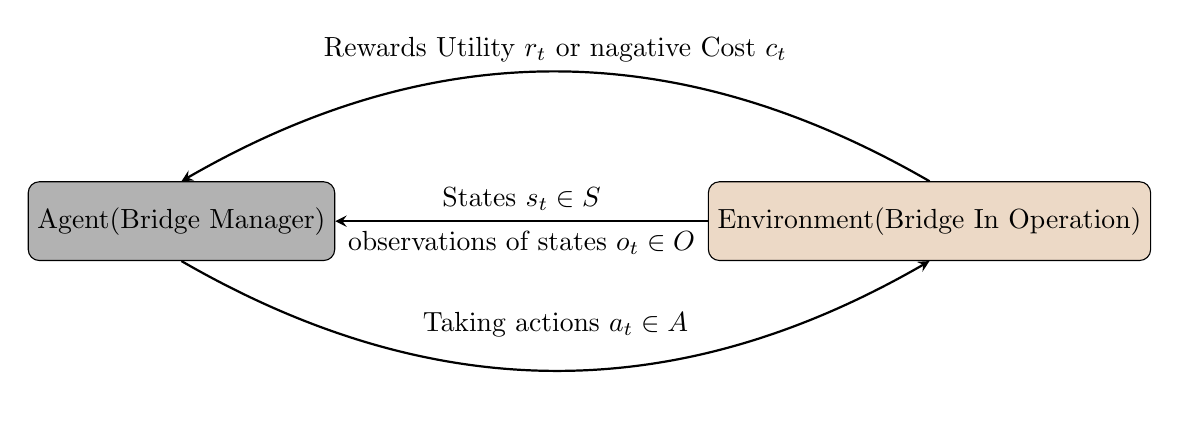
\begin{tikzpicture}[node distance=1.5cm]
	\node (Agent) [agent] {Agent(Bridge Manager) };
	\node (Env) [env, right of= Agent,xshift = 80mm] {Environment(Bridge In Operation)};	
	% First have some observations of states
	\draw [arrow] (Env) -- node[above]{States $s_t \in \mathds{S}$ } node[below]{observations of states $o_t \in \mathds{O}$}(Agent);
	% Then take actions according to the states or observations
	\draw [arrow] (Agent.south) to [out=-30,in=-150]node[above,yshift = 3mm]  {Taking actions $a_t \in \mathds{A}$} (Env.south);
	% Get feedback from the environment
	\draw [arrow] (Env.north) to [out=150,in=30]node[above] {Rewards Utility $r_t$ or nagative Cost $c_t$}  (Agent.north);
\end{tikzpicture}		
\end{document}